\chapter{\IfLanguageName{dutch}{Stand van zaken}{State of the art}}%
\label{ch:stand-van-zaken}

Zoals vermeld in het vorige hoofdstuk onderzoeken we oplossingen voor de problemen waarmee het bedrijf Lockit Rentals kampt. Alvorens deze oplossingen aangeboden worden, is het van belang om inzicht te verwerven van gebruikte technologieën. Om deze technologieën goed te doorgronden moet er bestudeerd worden welke hedendaagse technieken gehanteerd worden. De literatuurstudie is onderverdeeld in twee delen. Enerzijds het analyseren van een aangemaakte QR-code. Inclusief de uitwerking en de functionaliteit hoe deze QR-codes geïntegreerd zijn in de locker systemen. Het maken en integreren van een oplossing voor de verloren QR-code zal plaatsvinden in het tweede deel van de literatuurstudie. Door deze technologieën te bestuderen maken we gebruik van de verworven kennis om het oplossingsgericht onderzoek te starten.

\section{Wie is Lockit Rentals}%
\label{sec:lockitRentals}


Lockit Rentals is een naam onder het bedrijf VD Group BV. Deze is opgericht op 6 november 2019 door Sébastien Vandenhouten en Wannes Van Dorpe met als doel lockers te verhuren op evenementen. Enkele maanden na de oprichting begon de covid-19 crisis die de volledige sector tot stilstand deed komen. Na de crisis werd er direct geïnvesteerd in nieuwe lockers. Niet de gewone traditionele lockers, maar speciale technologische lockers die nog niet beschikbaar waren in België. De lockers werden in een mum van tijd omgebouwd tot QR-smart locker units met daarin lockers. Zo zijn er in het voorjaar van 2022, 13 units geproduceerd door Lockit Rentals. Op de dag van vandaag wordt er ijverig gezocht naar nieuwe investeerders om hun vloot van units uit te breiden.

Er zijn verschillende manieren om smart lockers systemen te gaan produceren. Hieronder volgt een opsomming van de verschillende smart lockers systemen elk met hun eigenschappen. Deze methodes zijn opgesteld door Lockit Rentals om hun marktonderzoek te starten.
\\
\textbf{Pincode:}
\begin{itemize}
    \item Kan vergeten worden
    \item Manuele verkoop mogelijk
    \item 100\% online verkoop mogelijk
    \item Trage verwerking bij openen van locker (pincode moet manueel worden ingetypt)
    \item Spieken is mogelijk waardoor er risico’s tot diefstal    
\end{itemize}

\textbf{Rfid Badge:}
\begin{itemize}
    \item Kan verloren gaan
    \item Manuele verkoop mogelijk
    \item Geen online verkoop mogelijk
    \item Snelle verwerking bij openen locker (scan en go)
    \item Spieken is niet mogelijk
    \item Fysiek object nodig + aankoop kost van badges    
\end{itemize}

\textbf{QR  code:}
\begin{itemize}
    \item Kan niet vergeten worden (kan ook niet onthouden worden)
    \item Manuele verkoop mogelijk
    \item 100\% online verkoop mogelijk
    \item Snelle verwerking bij openen lockers (scan QR-code en go)
    \item Spieken is niet mogelijk
    \item Technisch een veelvoud aan vereenvoudigingen mogelijk    
\end{itemize}

Uit deze korte opsomming van eigenschappen heeft Lockit Rentals besloten om zich te richten op het maken van lockers die openen op basis van een correcte QR code. Het gebruik van een QR code is vandaag de dag ook geen onbekend terrein. Door het mainstream maken van QR codes in betalingen, doorlinken van websites, covidsafe app, etc. zijn veel mensen al eens in aanraking gekomen met een QR-code \autocite{Belle2023}. Het gebruik van een QR code voor het openen van lockers is de logische stap voorwaarts \autocite{Lo2014}.
Uiteraard zijn ze niet de enige die smart locker systemen op de markt hebben. Enkele bedrijven die hier ook bij aanschuiven zijn, mobile lockers, LockerKing en Rental Group.

\section{Hoe zijn de QR-units opgebouwd}%
\label{sec:QR-units}
De smart locker systemen zijn toegankelijk met een geldige toegangscode die voorgesteld wordt als een QR-code. Het systeem bestaat uit verschillende soorten technologieën en elektronische componenten. De combinatie van hardware en software die nauw met elkaar samenwerken, vormen gezamenlijk één QR-unit \autocite{Jadhav2016} . De units hebben enkel 230 volt nodig om volledig operationeel te zijn. 

De hardware bestaat uit mechanische onderdelen zoals een deurslot \ref{fig:lockerSlot}, het volledige frame van de unit maar ook uit elektronische onderdelen zoals een camera, Raspberry Pi, digitaal scherm, etc. De mobiele applicatie waar de QR-codes kan verkocht worden en zo ook genereren, heeft geen verband met de interne werking van een QR-unit. Het enige dat de QR-unit nodig heeft, is een correct opgebouwde QR-code. Hiermee krijgt de festivalganger toegang tot zijn/haar gehuurde locker.

Elke unit bevat 128 lockers verspreid over 4 kasten zoals te zien op figuur \ref{fig:lockerUnit}. De locker units zijn waterdicht en dus optimaal voor plaatsing in niet overdekte locaties. Eén locker kast bevat 24 lockers, 4 grote die zich op de bovenste rij bevinden. De 20 overige zijn een iets kleiner formaat en situeren zich onderaan. De lange zijden van een QR-unit zijn uitklapbare luiken met aan elke kant twee kasten. Er zijn 4 kasten per unit aanwezig wat een totaal geeft van 128 lockers voorgesteld op figuur \ref{fig:lockerUnit} en  \ref{fig:lockerUnit2}.

\begin{figure}[h]
    \centering
    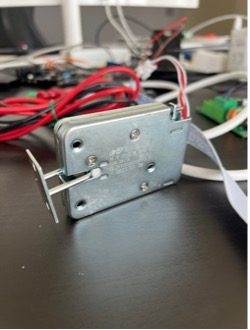
\includegraphics[height=7cm]{F1_lockerSlot.jpg}
    \captionsetup{justification=centering, singlelinecheck=false}    
    \caption{Een locker slot.}
    \label{fig:lockerSlot}
\end{figure}}

\begin{figure}[h]
    \centering
    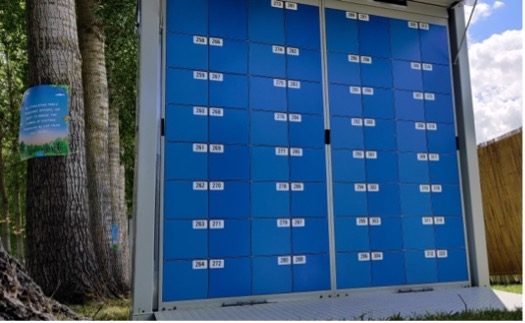
\includegraphics[height=6cm]{F2_lockerUnit.jpg}
    \captionsetup{justification=centering, singlelinecheck=false}    
    \caption{Reële weergave van een locker unit.}
    \label{fig:lockerUnit}
\end{figure}

\begin{figure}[h]
    \centering
    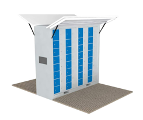
\includegraphics[height=7cm]{F3_lockerUnit2.png}
    \captionsetup{justification=centering, singlelinecheck=false}    
    \caption{Een uitgetekende weergave van een locker unit.}
    \label{fig:lockerUnit2}
\end{figure}}

\newpage

\section{Hoe is een QR-code opgebouwd}%
\label{sec:opbouwQR-code}

Een QR-code is een machinaal leesbaar optisch label met informatie over het bijhorende product \autocite{Chang2014}. In deze context wordt het product als toegangscode gebruikt. QR-code staat voor Quick Response code en is een matrix van de welbekende streepjes code \autocite{Tiwari2016}. Het is een tweedimensionale code die informatie zoals tekst, URL of andere data bevat  \autocite{Shin2012} \autocite{Baharav2013}. In ons geval is het dus informatie die toebehoort bij een overeenkomstige locker. De QR-code is zodanig ontworpen dat ze door een smartphone uitgelezen kan worden aan hoge snelheden \autocite{Tiwari2016}. Dit maakt het optimaal als de QR-code gebruikt wordt als toegangscode \autocite{Narang2012}. De grootte van de QR-code kan aangepast worden naarmate de hoeveelheid data die hierin gestockeerd moet worden \autocite{Tiwari2016}. 
\\
Een QR-code wordt opgebouwd en voorgesteld als een vierkant \autocite{Fujita2011}. Hierrond bevindt zich een witte omranding. Dit vormt een contrast zodat de QR-scanner minder moeite heeft om de oppervlakte uit te lezen \autocite{Wang2015}. Dit is 1 van de 7 cruciale eigenschappen. Plaats markeringen zijn aanwezig om de scanner een duiding te geven hoe de code is gepositioneerd. Uitlijnmarkeringen hebben eveneens dezelfde functie maar deze zijn meer van toepassing bij grote QR-codes. De QR-code bevat timing patronen, dit zijn lijnen die de scanner vertellen hoe groot de data matrix is. De twee belangrijkste elementen van een QR-code zijn gegevens en foutcorrectiesleutels. Hierin zit de data gecapteerd inclusief de informatie hoe het algoritme moet omgaan met fouttolerantie \autocite{Tiwari2016}  \autocite{Petrova2016}  \autocite{Li2018}). Op figuur \ref{fig:voorstellingQR} zie je een visuele weergave. 
De fouttolerantie is doorslaggevend indien de QR-code gebruikt wordt als toegangscode \autocite{Tiwari2016}.  De fouttolerantie kan ingesteld worden door configuratie toe te passen. Het kan ingesteld worden op vier levels beginnend bij fouttolerantie van 7\% tot 30\% \autocite{Tiwari2016}.

\begin{figure}[h]
    \centering
    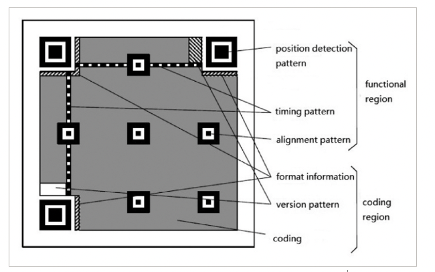
\includegraphics{F4_voorstellingQrCode.png}
    \captionsetup{justification=centering, singlelinecheck=false}    
    \caption{Een technische voorstelling van een QR-code.}
    \label{fig:voorstellingQR}
\end{figure}}

De voordelen van de QR-codes vormen een duidelijk beeld waarom Lockit Rentals voor deze technologie gekozen heeft. Niet enkel naar functionaliteit en flexibiliteit toe maar eveneens is het een makkelijk traceerbare tool. Bij verkoop van QR-codes kan men een overzicht opmaken hoeveel QR-codes er effectief gegenereerd zijn. Op basis van deze gegevens kunnen verkoopcijfers makkelijk berekend worden. 

De kans op diefstal wordt ook alsmaar kleiner als de toegangscode bestaat uit elementen die niet waarneembaar zijn \autocite{Baharav2013}. Hoe minder de persoon in kwestie weet over de code hoe moeilijker deze is om door te geven aan anderen ook al is het niet hun intentie.

\newpage
\subsection{Stappenplan voor de ontwikkeling en verkoop van QR-codes}%
\label{sec:opbouwQR-codeVerkoop}

Het proces voor het genereren van QR-codes van de mobiele applicatie wordt vooraf gegaan door allerlei fases. De aangekochte QR-code aanmaken en weergeven naar de klant is de laatste fase in het proces. De applicatie kan meerdere versies van QR-codes genereren elk met hun eigen doel en eigenschappen. Zo bestaan er QR-codes die de software automatisch updaten of een universele QR-code die automatisch alle lockers kan openen. Deze QR-codes zullen gehanteerd worden door logistieke medewerkers. Hieronder volgen de vier stappen van het proces met als einddoel de QR-code aan te maken.

\begin{comment}
    Hoewel een QR-code een standaard grafische voorstelling is, kan de grootte van een code verschillen. Wanneer een code groter is, ontstaat er meer witruimte tussen de pixels \autocite{Li2018}. Hierdoor kan de camera de code makkelijker en sneller scannen \autocite{Karrach2020}. Ook de foutcorrectie zorgt ervoor dat de resolutie vergroot zal worden. Hoe groter de resolutie van de QR-code hoe meer data gestockeerd kan worden \autocite{Chow2016}. 
\end{comment}


\subsubsection{Stap 1: Gegevens en voorkeur klant verwerven}%
\label{sec:opbouwQR-codeVerkoop1}

\textit {De toelichting die hieronder weergeven wordt, is een vereenvoudigde voorstelling van de effectieve implementatie. Dit onderdeel van de toepassing is niet het hoofdonderwerp van deze bachelorproef, op deze analogie wordt niet verder ingegaan.}

\vspace{7}
De gegevens van de klant worden opgevraagd als hij/zij een QR-code wenst te kopen. Aan de hand van deze gegevens wordt er een gebruikersaccount automatisch aangemaakt en worden de gegevens bijgehouden \ref{lst:ophalenUser}. Deze aanpak maakt het mogelijk om nadien een koppeling te leggen tussen lockernummer en gebruiker. De reservatie en tot stand brengen van een QR-code zijn twee aparte concepten.
\begin{lstlisting}[caption={Ophalen de zopas aangemaakte gebruiker zijn gegevens indien hij in het huur proces terecht gekomen is.}, label={lst:ophalenUser}]
    /**
    * Get the user auth uid
    */
    const userAuthUid: string | undefined = context.auth?.uid;
    
    if (!userAuthUid) {
        functions.logger.error('No authenticated user was found', { data: data });
        throw new functions.https.HttpsError(
        'invalid-argument',
        'Something went wrong authenticating your device.'
        );
    }
    
    /**
    * If this user is registerd, get his info
    */
    let user: User;
    if (context?.auth?.token.email) {
        const userd = await db.collection('users').doc(userAuthUid).get();
        user = userd.data() as User;
    }
\end{lstlisting}

Bij het huurproces van een locker moet een huurder het festival aanduiden waar hij/zij de locker wil huren. Niets sluit uit dat de lockers operationeel zijn op twee verschillende locaties. Daarna heeft de huurder de keuze om het formaat te selecteren en als deze optie beschikbaar is hoelang de huurtijd zal zijn. Echter is het verstrijken van deze details over het geselecteerde evenement noodzakelijk voor de opbouw van de QR-code. De QR-code wordt gegenereerd op basis van de beschikbare lockers die aanwezig zijn op het geselecteerde evenement \ref{lst:ophalenEventInfo}.

\begin{lstlisting}[caption={Het informatie ophalen van de geselecteerde locatie. Aan de hand van geselecteerde evenement kan er gegevens uit de databank gehaald worden.}, label={lst:ophalenEventInfo}]
    /**
    * Get more info about the shop
    */
    const shopSnap = await db.collection('shop').doc(data.shopId).get();
    const shop: Shop = shopSnap.data() as Shop;
    
    /**
    * Check if selected option is active in shop
    */
    if (!shop.activeOptions?.find((o) => o.optionId === data.optionId)) {
        functions.logger.error(
        'Attempting reservation creation for non-active option',
        { data: data }
        );
        throw new functions.https.HttpsError(
        'invalid-argument',
        'This option is not yet active.'
        );
    }
    
    /**
    * Get more info about the option and location
    */
    const optionSnap = await db
    .collection('shop')
    .doc(data.shopId)
    .collection('options')
    .doc(data.optionId)
    .get();
    const option: ShopOption = optionSnap.data() as ShopOption;
    
    if (!option) {
        functions.logger.error('Can not find option for id', { data: data });
        throw new functions.https.HttpsError(
        'invalid-argument',
        'Something went wrong.'
        );
    }
    
    const locationSnap = await db
    .collection('shop')
    .doc(data.shopId)
    .collection('locations')
    .doc(option.location)
    .get();
    const location: ShopLocation = locationSnap.data() as ShopLocation;
    
    if (!location) {
        functions.logger.error('Can not find location for id', { data: data });
        throw new functions.https.HttpsError(
        'invalid-argument',
        'Something went wrong.'
        );
    }
\end{lstlisting}

\subsubsection{Stap 2: De reservatie voor een toegangscode van een locker}%
Op voorwaarde dat de gebruiker informatie geldig is en er nog een locker beschikbaar is, zal er een reservatie aangemaakt worden en meteen bewaard worden in een databank. Het code die hiervoor verantwoordelijk is wordt afgebeeld in listing \ref{lst:aanmakenReservatie}.

\begin{lstlisting}[caption={De creatie van een reservatie voor het huren van een locker. Deze reservatie wordt bijgehouden in de databank}, label={lst:aanmakenReservatie}]
    /**
    * Create the reservation
    */
    const createdReservationRef = db
    .collection('shop')
    .doc(data.shopId)
    .collection('reservations')
    .withConverter(converter<ShopReservation>())
    .doc();
    
    await transaction.set(createdReservationRef, {
        id: createdReservationRef.id,
        /**
        * Here we decide if the reservation should be filled asap without payment or if a payment is needed
        */
        status: determineReservationStatus(option, data, context, user),
        customerAuthId: userAuthUid,
        customerOrigin: context.rawRequest.headers.referer,
        customerEmail: data.customerEmail,
        customerName: data.customerName,
        customerPhone: data.customerPhone,
        lockerType: data.lockerType,
        shopId: shopSnap.id,
        shopName: shop.name,
        shopAvatar: shop.avatar,
        optionColor: option.color,
        optionId: optionSnap.id,
        optionLocationId: locationSnap.id,
        optionLocationName: location.name,
        optionName: option.name,
        optionPeriodFrom: option.periodFrom,
        optionPeriodTo: option.periodTo,
        optionType: option.optionType,
        priceToPay: option.pricePerType[data.lockerType],
        manual: !!data.manual,
        reservationCreated: moment().unix(),
    });
    
    return Promise.resolve(createdReservationRef);
});
\end{lstlisting}

\subsubsection{Stap 3: Het betalingsverzoek voor een toegangscode van een locker}%
\label{sec:opbouwQR-codeVerkoop12}

Wanneer de databank een nieuwe reservatie constateert, wordt er een trigger uitgevoerd. Een trigger is een procedure die verplicht uitgevoerd wordt als een welbepaalde tabel een aanpassing ondergaat \autocite{documentation}. In dit geval is het de tabel ‘reservations’. Deze trigger zal een methode aanroepen om het betalingsverzoek te gecreëeren. 
De logistieke medewerkers kunnen huurders helpen indien hun QR-code te hard beschadigd is of als ze hun toegangscode tot de locker verloren zijn. Bij het aanmaken van toegangscodes bij logistieke medewerkers verloopt het proces op een alternatieve wijze.  Deze springen over het betalingsproces en verwerven direct een geldige QR-code. Zonder de aangemaakte betaling veld in de databank op te slaan.  \ref{lst:aanmakenBetaling}

\begin{lstlisting}[caption={Valideert of er een betaling van toepassing is. Indien nodig creëert het een betaling en bewaard deze in de databank}, label={lst:aanmakenBetaling}]
    /**
    * No action is needed but to move the status along
    */
    if (createdReservation.status === ReservationStatus.NO_PROVIDER_NEEDED) {
        await snap.ref.update({
            status: ReservationStatus.OPEN,
        });
    }
    
    /**
    * A payment is needed
    */
    if (createdReservation.status === ReservationStatus.WAITING_FOR_PROVIDER) {
        const mollieApiKey = process.env.MOLLIE_API_KEY || '';
        
        const mollie = await createMolliePayment(mollieApiKey, createdReservation);
        
        /**
        * Create the payment
        */
        const paymentRef = db
        .collection('shop')
        .doc(createdReservation.shopId)
        .collection('payments')
        .withConverter(converter<ShopPayment>())
        .doc();
        
        await paymentRef.set({
            id: paymentRef.id,
            reservationId: createdReservation.id,
            customerEmail: createdReservation.customerEmail,
            customerName: createdReservation.customerName,
            customerPhone: createdReservation.customerPhone,
            lockerType: createdReservation.lockerType,
            optionColor: createdReservation.optionColor,
            optionId: createdReservation.optionId,
            optionLocationName: createdReservation.optionLocationName,
            optionName: createdReservation.optionName,
            priceToPay: createdReservation.priceToPay,
            shopName: createdReservation.shopName,
            status: ShopPaymentStatus.PENDING,
            provider: PaymentProvider.MOLLIE,
            mollieData: {
                id: mollie.id,
            },
        });
\end{lstlisting}

De tool Mollie is een online betalingsservice die wordt gehanteerd om de betalingen succesvol af te ronden \autocite{docs2023}. Gelijktijdig met de betaling wordt er een interne teller bijgehouden zodat deze locker geblokkeerd wordt voor andere kopers. Als de betaling niet succesvol is, wordt de locker terug vrijgegeven na een bepaalde periode. De betaling word aangemaakt met de gekende informatie over de gewenste locker \ref{lst:aanmakenBetalingMollie}.

\begin{lstlisting}[caption={Mollie betaling aanmaken met nodige data.}, label={lst:aanmakenBetalingMollie}]
    async function createMolliePayment(
    mollieApiKey: string,
    reservation: ShopReservation
    ): Promise<Payment> {
        const mollieClient = createMollieClient({
            apiKey: mollieApiKey,
        });
        return mollieClient.payments.create({
            amount: {
                value: reservation.priceToPay.toFixed(2),
                currency: 'EUR',
            },
            description:
            reservation.shopName +
            ' | ' +
            reservation.optionName +
            ' | ' +
            reservation.lockerType,
            redirectUrl: reservation.customerOrigin + 'reservations/' + reservation.id,
            webhookUrl:
            reservation.customerOrigin?.includes('localhost') ||
            reservation.customerOrigin?.includes('test')
            ? 'https://europe-west2-lockit-testing.cloudfunctions.net/mollieWebhook'
            : 'https://europe-west2-lockit-435cd.cloudfunctions.net/mollieWebhook',
            metadata: {
                shop: reservation.shopName,
                reservation: reservation.id,
                option: reservation.optionName,
                location: reservation.optionLocationName,
                lockerType: reservation.lockerType,
                customer: reservation.customerName,
                customerEmail: reservation.customerEmail,
                customerPhone: reservation.customerPhone,
            },
        });
    }
    \end{lstlisting}

Bij correcte betaling van de klant, zal de applicatie de desbetreffende creatiemethode aanspreken om dergelijke QR-code te genereren. Deze QR-code bevat een random geselecteerde locker nummer inclusief een tijdspanne waarin de toegangscode geldig is. De status van de reservatie die zich al in de databank bevindt ,wordt aangepast. Hierdoor weet heel de applicatie dat die bepaalde reservatie betaald is \ref{lst:voltooidebetaling}.


\begin{lstlisting}[caption={Voltooide betaling roept de creatie QR-code methode op. Hierbij gebeurt een status update van de vooraf aangemaakte reservatie.}, label={lst:voltooidebetaling}]
    await db.runTransaction(async (transaction) => {
        /**
        * Find a valid available locker
        * Because we can only compare 10 units with the firestore "IN" clause we have to split up
        */
        
        if (!location?.units) {
            throw new Error('No units assigned');
        }
        
        const availableLockerSnap = await getRandomLockerAvailable(
        transaction,
        db,
        reservation.lockerType,
        location?.units
        );
        if (!availableLockerSnap) {
            logger.error('no-open-locker-found', {
                reservation: reservation,
                option: option,
                location: location,
            });
            throw new Error('NO Open lockers found');
        }
        
        const generatedCode = await generateQrCodeWithRecordOnTransaction(
        transaction,
        {
            lockerNumber: availableLockerSnap.data().number,
            start: option?.periodFrom as number,
            end: option?.periodTo as number,
            color: option?.color as string,
            image: reservation?.shopAvatar,
            location: location?.name,
            periodName: option?.name as string,
            name: reservation?.shopName,
        }
        );
        
        /**
        * update current reservation
        */
        await transaction.update(reservationSnap.ref, {
            status: ReservationStatus.FILLED,
            accessCode: generatedCode,
            lockerNumber: availableLockerSnap.data().number,
        });
\end{lstlisting}

\newpage
\subsubsection{Stap 4: Creatie QR-code na succesvolle betaling}%
\label{sec:opbouwQR-codeVerkoop123}

Om de QR-code te tonen op de mobiele applicatie hebben we componenten nodig om de gegenereerde QR-code visueel te tonen zoals op figuur \ref{fig:qrCodeGebruiker} of figuur \ref{fig:qrCodeAdmin}. Hierdoor kan de koper zowel de code scannen op zijn/haar telefoon als op een afgedrukt kaartje \autocite{Chow2016}.

\begin{figure}[h]
    \centering
    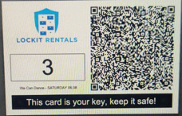
\includegraphics{F5_qrcodeKoper.png}
    \captionsetup{justification=centering, singlelinecheck=false}    
    \caption{Een voorbeeld van een QR-code die gekocht is door een gebruiker voor specifieke lockertoegang op een evenement.}
    \label{fig:qrCodeGebruiker}
\end{figure}}

\begin{figure}[h]
    \centering
    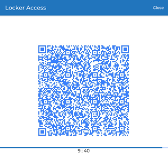
\includegraphics{F6_qrcodeAdmin.png}
    \captionsetup{justification=centering, singlelinecheck=false}    
    \caption{Een voorbeeld van een QR-code die gegeneerd is door een logistieke medewerker met de juiste bevoegdheden voor specifieke lockertoegang op een evenement.}
    \label{fig:qrCodeAdmin}
\end{figure}}

Aangezien de generatie van een QR-code dat voorgesteld is als afbeelding wat front-end matige materie is, zal onderstaande code de werking weergeven \ref{lst:qrComponent}. 

\begin{lstlisting}[caption={Typescript code voor een visuele QR-code aan te maken}, label={lst:qrComponent}]
    await db.runTransaction(async (transaction) => {
        export class QrcodeViewerComponent implements OnInit {
            activeQrCode: string = 'EjIQT51wpdf6Is1r+R5+mt8aU0waHVKVK9lzvhXRV4w=';
            
            @Input() data: string = '';
            @Input() deCryptedData: QrCodeData = QrCodeData.createEmptyQrCodeData();
            
            secondsLeft$: Observable<number> = new BehaviorSubject(0);
            
            private qr_opts = {
                errorCorrectionLevel: 'H',
                type: 'image/jpeg',
                quality: 1,
                margin: 10,
                color: {
                    dark: '#3880ff',
                },
            };
            
            constructor(private modalController: ModalController) {
                this.secondsLeft$ = interval(1000).pipe(
                filter(
                () => !!this.deCryptedData.validFrom && !!this.deCryptedData.validTo
                ),
                map(() => this.deCryptedData.getSecondsLeftUntilEnd())
                );
            }
            
            ngOnInit(): void {
                qrcode
                .toDataURL(this.data, this.qr_opts as QRCodeToDataURLOptions)
                .then((qr) => {
                    this.activeQrCode = qr;
                });
            }
            
            dismissModal() {
                this.modalController.dismiss();
            }
        }
    \end{lstlisting}

Lijn 3: De variabele ‘activeQrCode’ van type string is de publieke sleutel die wordt gebruikt om de QR-code te ontcijferen. \\
Lijn 10 – 18: De ingestelde eigenschappen die gedefinieerd zijn om de QR-code aan te maken. Men kan de code naar zijn behoefte configureren \autocite{Sutheebanjard2010}. Een belangrijke waarde is hierbij de ‘ErrorCorrectionLevel’, deze veranderd doorheen de applicatie op basis waar de QR-code afgebeeld moet worden. Hierdoor mag de QR-code voor 30\% beschadigd of gescheurd zijn. De scanner zal alsnog de afbeelding succesvol kunnen detecteren \autocite{Tiwari2016}. \\
Lijn 29– 35: De tool die gehanteerd wordt om de QR-code te genereren is de bibliotheek ‘qrcode’ \autocite{pypi2023}. 

\newpage
\section{Het incrypteren en decrypteren van QR-codes}%
\label{sec:encryptQR-code}

Eerder in de werking van de QR-units is de validatie NaCL genaamd ‘Networking And Cryptography Library’ aan bod gekomen \autocite{Bernstein}. De hoofdfunctionaliteit van de recente software bibliotheek is het vercijferen en ontcijferen van bestanden. Het biedt alle kernbewerkingen aan die betrekking hebben om cartografische benodigdheden op hoger niveau te bouwen \autocite{Bernsteina}.

In de applicatie van Lockit Rentals is er gebruik gemaakt van TweetNaCl.js. TweetNaCl is een compacte versie van de implementatie bibliotheek NaCL \autocite{Bernstein2014} \autocite{Bernsteinb}. Deze bevat verschillende encryptie en onderteken algoritmes op basis van ed25519 \autocite{Bernstein2011}. \\
Ed25519 gebruikt het onderliggende algoritme Curve25519. Curve25519 is vooral ontworpen om snel, efficiënt en op een effectieve manier sleutelwisseling te gaan uitvoeren. Zo worden beide partijen op de hoogte gesteld van hun gezamenlijke sleutel \autocite{Bernstein2006}. Ed25519 aan de andere kant heeft andere prioriteiten. Deze zal op een betere en sneller manier algoritmen uitvoeren specifiek voor digitale ondertekeningen gaan uitvoeren. \autocite{Bernstein2011}. \\
In het kader van smart locker systemen wordt de encryptie gebruikt om de QR-codes digitaal te ondertekenen. De reden van gebruik ligt bij een voordeel van TweetNaCL.js die heel voordelig uitkomt bij de gegeven implementatie. Het heeft namelijk als voordeel dat deze beschikt over kleine onderteken sleutels ook wel ‘signatures’ genoemd \autocite{Bernstein2011}. Hoe minder gestockeerde data in de QR-code kleiner de afdruk is van de code \autocite{Chow2016}.

Deze term van algoritme wordt ‘signing’ genoemd. Het algoritme zal verifiëren of de data in de QR-code onveranderd blijft gedurende het gehele proces \autocite{Bernsteinb}. Het proces begint bij het tot stand brengen van een QR-code tot aan het scannen ervan.

De documentatie website van TweetNaCl.js laat de verschillende encryptie tool gratis uitproberen \autocite{Bernsteinb}. Een concreet voorbeeld hieronder geeft duiding hoe een specifiek bericht ondertekend kan worden. Hieruit kan aangetoond worden of het bericht al dan niet is aangepast na de creatie \autocite{Bernstein2014}.

\subsection{Uitgewerkt voorbeeld met digitale ondertekening op een standaard bericht}%
\label{sec:voorbeeldDigitaleSigning}

Bij het ondertekenen van een bericht heeft het algoritme nood aan één geheime sleutel evenals één publieke sleutel
\ref{fig:privatePublicKey}. De geheime sleutel wordt gebruikt om nadien de versleutelde code te decrypteren.

\begin{figure}[h]
    \centering
    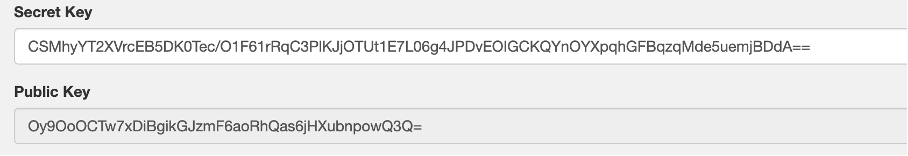
\includegraphics{F7_privatePublicKeys.png}
    \captionsetup{justification=centering, singlelinecheck=false}    
    \caption{De publieke en private sleutel voor encryptie aan de hand van TweetNaCL.js.}
    \label{fig:privatePublicKey}
\end{figure}}
 \newpage
In deze illustratie wordt een bericht dat afgebeeld staat hieronder \ref{fig:encryptionBericht} meegegeven met de functie van TweetNaCl. Met als doel dit bericht te laten ondertekenen aan de hand van de geheime sleutel.

\begin{figure}[h]
    \centering
    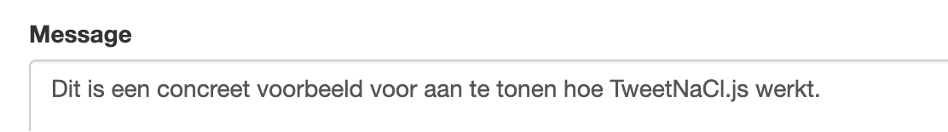
\includegraphics{F8_messageEncryption.png}
    \captionsetup{justification=centering, singlelinecheck=false}    
    \caption{Het bericht dat cryptisch ondertekend moet worden aan de hand van TweetNaCL.js.}
    \label{fig:encryptionBericht}
\end{figure}}

Bij ondertekening van dit bericht ontstaat er een unieke handtekening  \ref{fig:signatureQrcode} als zijnde een tekenreeks. Aan de hand van deze code kan de ontvanger verifiëren dat het bericht gedurende het proces niet gewijzigd is.

\begin{figure}[h]
    \centering
    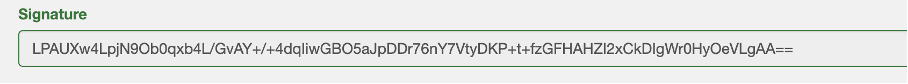
\includegraphics{F9_signature.png}
    \captionsetup{justification=centering, singlelinecheck=false}    
    \caption{De gegenereerde digitale handtekening aan de hand van TweetNaCL.js}
    \label{fig:signatureQrcode}
\end{figure}}

\subsection{Verificatie van ondertekend bericht}%

Om na te gaan of dit bericht zijn oorspronkelijke data bevat zal de functie ‘verify’ opgeroepen worden. In het geval dat dit bericht niet in oorspronkelijke status bevindt, zal de functie een foutboodschap retourneren \ref{fig:verifyFailed}. Als de methode geen foutboodschap weergeeft, kan men concluderen dat deze data origineel is \autocite{Bernstein2014}. Zoals word weergegeven in figuur \ref{fig:verified}.

\begin{figure}[h]
    \centering
    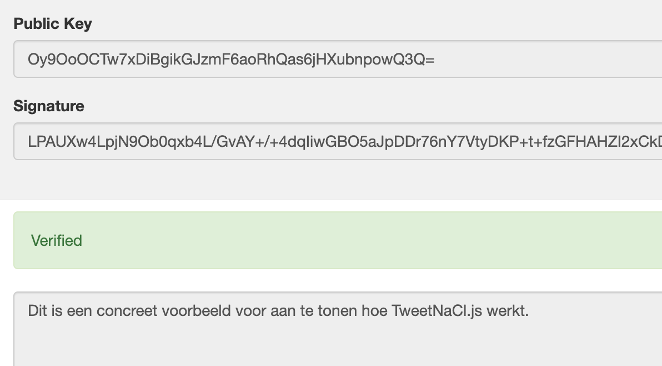
\includegraphics{F10_verified.png}
    \captionsetup{justification=centering, singlelinecheck=false}    
    \caption{Bewijs dat bericht zich in originele  staat bevindt.}
    \label{fig:verified}
\end{figure}}

\begin{figure}[h]
    \centering
    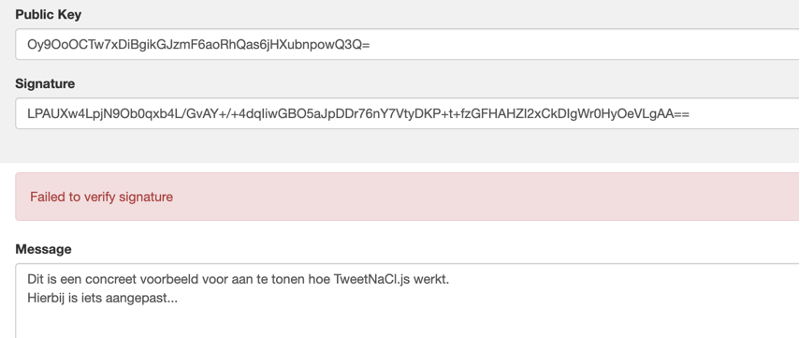
\includegraphics{F11_failedVerify.png}
    \captionsetup{justification=centering, singlelinecheck=false}    
    \caption{Bewijs dat bericht zich in geen originele  staat bevindt.}
    \label{fig:verifyFailed}
\end{figure}}
\\
\newpage
\newpage
\subsection{Uitgewerkt voorbeeld van digitale ondertekening op een aangemaakte QR-Code.}%
\label{sec:voorbeeldDigitaleSigningQRCode}

Bij de implementatie van deze smart locker technologie is het bericht dat standaard meegegeven wordt de QR-code data van type \ac{JSON} object. Deze kan niet ondertekend worden zolang het niet geconverteerd wordt naar een tekstueel gegeven. De omvorming van een \ac{JSON} object naar een string wordt verwerkt door de functie ‘deCodeBase64’. Deze functie zal de reeks decoderen terug naar het oorspronkelijke binair formaat \autocite{Josefsson2006}.



\begin{lstlisting}[caption={Data object met de naam smallItem bevat de essentiele data om een locker te openen.}, label={lst:essentieleQrdata}]
    export async function generateQrCodeWithRecord(qrData: {
        lockerNumber: any;
        start: number;
        end: number;
        color: string;
        image: string;
        location: string;
        name: string;
        periodName: string;
    }) {
        const smallItem = convertToSmallPayload(
        qrData.lockerNumber,
        qrData.start,
        qrData.end
        );
\end{lstlisting}

Lijn 11 - 15 \ref{lst:essentieleQrdata} :  De data die essentieel is om toegang te hebben tot de locker wordt gedefinieerd als de variabele ‘smallItem’. Aangezien de eigenschappen zoals kleur, locatie en afbeelding niets te maken heeft met de scanfunctie van de QR-unit. Word deze informatie hiervan gescheiden.

De functie ‘NaCL. Sign()’ aanvaardt twee parameters \ref{lst:encryptionCode}. In de eerste plaats nemen we de locker informatie op. Deze informatie beschikt over de locker nummer, creatiedatum QR-code en verval datum QR-code \ref{lst:essentieleQrdata}. Het is noodzakelijk dat het tekstbericht het juiste type is daarom wordt ‘smallItem’ omgezet naar een JSON object en daarna geconverteerd naar byte door de functie ‘decodeUTF8()’. Vervolgens heeft de functie een geheime sleutel nodig om de ondertekening te kunnen uitvoeren.

\begin{lstlisting}[caption={Digitale ondertekening van QR-code data.}, label={lst:encryptionCode}]
    const data = nacl.sign.detached(
    decodeUTF8(JSON.stringify(smallItem)),
    decodeBase64(
    'Hier komt de private key.'
    )
    );
    \end{lstlisting}


Door de twee gecreëerde objecten, QR-data en de digitale handtekening samen te voegen ontstaat er een \ac{JSON} object genaamd ‘createdCode’ \ref{lst:createCode}. De code wordt achteraf omgevormd naar een tekstueel formaat.

\begin{lstlisting}[caption={Samenstellen van object, locker informatie en verificatie code.}, label={lst:createCode}]
    const createdCode = Buffer.from(
    JSON.stringify({ d: smallItem, v: encodeBase64(data) })
    ).toString('base64');
\end{lstlisting}

\newpage
\subsection{Verificatie van QR-code}%
\label{sec:controleaangemaakteQRcode}

Als illustratie maken we een QR-code aan op de applicatie die bestemd is voor locker nummer één. De geldigheidsduur van de code is tien minuten. Het request kan onderschept worden om zo de data te analyseren. We beelden het object af in figuur \ref{fig:dataobjectQR}.

\begin{figure}[h]
    \centering
    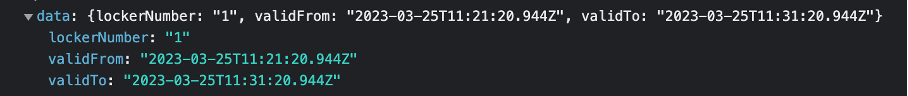
\includegraphics{F12_requestQrCode.png}
    \captionsetup{justification=ce/brntering, singlelinecheck=false}    
    \caption{Het data object bij de creatie van locker nummer 1 als logistieke medewerker. Deze heeft een tijdspanne van tien minuten.}
    \label{fig:dataobjectQR}
\end{figure}}

Als we dieper in de materie duiken is de aangemaakte code zichtbaar als antwoord op het creatieverzoek. De tekstuele code voorgesteld als base64 string ziet er als volgt uit: \\
 “eyJkIjp7Im4iOiIxIiwiZiI6MTY3OTc0MzIyMSwidCI6MTY3OTc0Mzg4MX0sInYiOiJLYT\\
 cwTmg4WUo3RlY0NmNiKythNlN3b21vczFFVURiQlpxajl2ZDhpNlNUWGZHU003eVN\\
 2ZGw0ZEs5WGp3clpyVnNV RlpHR3E3RVJGSlJQR09HTkxEdz09In0=".
 
\vspace{7}

Deze code wordt achter een vaste ingestelde URL geplaatst zodanig dat de QR-code gemakkelijk gedeeld kan worden. Het delen of doorsturen van een QR-code is een eenvoudig proces voor de huurder \ref{lst:shareQR}. Bij het delen van een QR-code wordt er een link gecreëerd dat verwijst naar de web applicatie van Lockit Rentals \ref{lst:createQRLink}. De applicatie zal de base64 string ontvangen en de link ontcijferen om zo een afbeelding van de QR-code genereren.

\begin{lstlisting}[caption={Het doorsturen van een QR-code in de vorm van een link.}, label={lst:shareQR}]
    handler: async () => {  
        await Share.share({
            title: 'Have access to my locker',
            text: 'Hi there, I want to share my locker with you. Open this link!',
            url: this.constructQRCodeData(qrData as string),
            dialogTitle: 'Share your locker with friends',
        });
\end{lstlisting}

\begin{lstlisting}[caption={De manier hoe de link van de QR-code is gestructureerd.}, label={lst:createQRLink}]
    constructQRCodeData(encryptedPart: string): string {
        return location.protocol + '//' + location.host + '/?code=' + encryptedPart;
    }
\end{lstlisting}

Op de figuur \ref{fig:decoderBase64ToJson} wordt een base64 van het type string omgevormd en ontcijferd  naar een tekstuele vorm. Hiervoor kan er gebruik gemaakt worden van gratis online tools. Om het base64 formaat te ontcijferen bestaat er een online decoder \autocite{base64decode}. 


\begin{figure}[h]
    \centering
    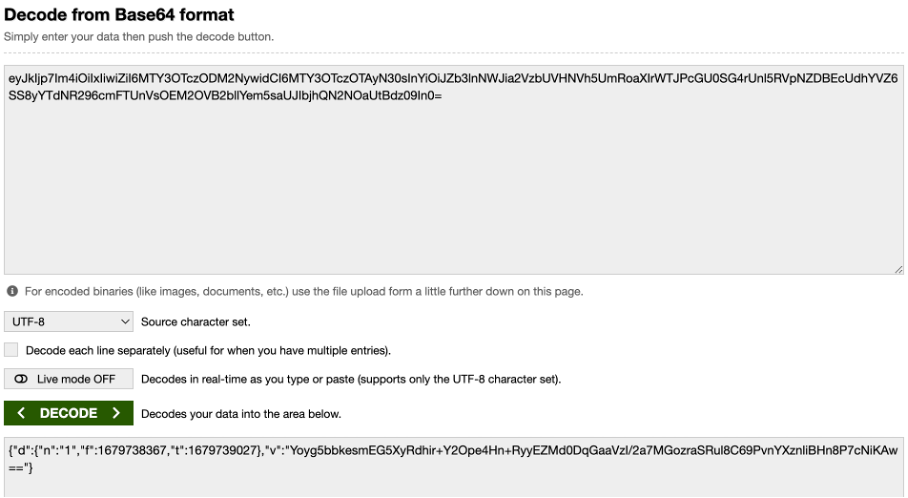
\includegraphics{F13_decoderbase64.png}
    \captionsetup{justification=ce/brntering, singlelinecheck=false}    
    \caption{De manier waarop een base64 string geconverteerd word naar een \ac{JSON} aan de hand van een online decoder.}
    \label{fig:decoderBase64ToJson}
\end{figure}}

Voor eenvoud van het illustratief voorbeeld vormen we dit om naar een gestandaardiseerd \ac{JSON} object \autocite{Concept}. Het geformatteerd \ac{JSON} object geeft een visueel beeld van de twee variabelen in de genereerde QR-code. Het visueel beeld word afgedrukt in de figuur \ref{fig:formattedJsonData}.

\begin{figure}[h]
    \centering
    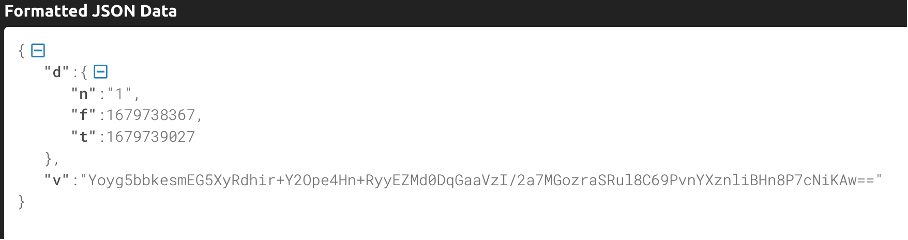
\includegraphics{F14_formattedJsonData.png}
    \captionsetup{justification=ce/brntering, singlelinecheck=false}    
    \caption{Het JSON object converteren naar een gestandaardiseerde vorm.}
    \label{fig:formattedJsonData}
\end{figure}

\newpage
Om de data te controleren wordt de functie ‘verify’ aangeroepen \ref{lst:verifyMethode}, deze heeft 3 parameters nodig. Als eerste het object waarin de QR-code data zit. Vervolgens geven we de verificatie code mee. De publieke sleutel is de laatste parameter om te decrypteren.


\begin{lstlisting}[caption={De controle van QR-code data met de TweetNaCL.js verifieer functie.}, label={lst:verifyMethode}]
    // Check if the object validates
    if (
    !nacl.sign.detached.verify(
    decodeUTF8(JSON.stringify(obj.d)),
    decodeBase64(obj.v),
    decodeBase64(publicKey)
    )
    ) {
        return new Error();
    }
\end{lstlisting}

Als data zijn originele vorm heeft aangehouden, zal de functie geen foutboodschap geven zoals in figuur \ref{fig:qrdataVerified}. Bij onveranderlijke data kan er van uitgegaan worden dat de QR-code informatie niet aangepast is doorheen het proces \autocite{Bernsteinb}. 

\begin{figure}[h]
    \centering
    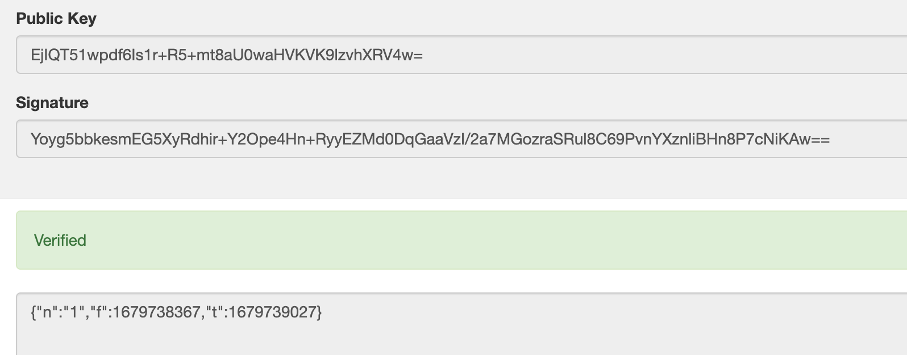
\includegraphics{F15_qrcodeVerified.png}
    \captionsetup{justification=ce/brntering, singlelinecheck=false}    
    \caption{De QR-code data dat vanaf de aanmaak tot de verifieer  functie ongewijzigd is gebleven.}
    \label{fig:qrdataVerified}
\end{figure}

\newpage

\section{Detecteren van QR-codes}
\label{sec:detecterenQr-codes}

De populariteit van QR-codes verplicht de omgeving zich aan te passen om deze twee dimensionale codes op een veilige en correcte manier snel uit te lezen. Het streven naar betere en snellere QR-code scanners is bij grote bedrijven essentieel \autocite{Ertekin2015}.
Om de problematiek van Lockit Rentals over de QR-code herkenning onder de loep te nemen, kijken wij naar hun gebruikte technieken om QR-codes te detecteren. Figuur \ref{fig:zijkantLocker} en \ref{fig:usbcameraLocker} toont aan dat het scannen van een QR-code gebeurt aan de hand van een USB camera. Om te scannen in donkere omgevingen hebben ze hierbij ook een lichtbron bij de scanner geplaatst.

\begin{figure}[h]
    \centering
    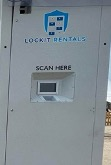
\includegraphics{F20_ZijkantLocker.jpg}
    \captionsetup{justification=ce/brntering, singlelinecheck=false}    
    \caption{Het vooraanzicht van een QR-unit met camera en digitaal scherm.}
    \label{fig:zijkantLocker}
\end{figure}

\begin{figure}[h]
    \centering
    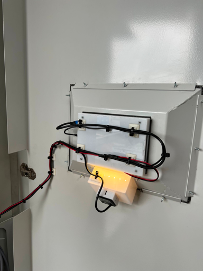
\includegraphics{F21_LockerUSBCamera.png}
    \captionsetup{justification=ce/brntering, singlelinecheck=false}    
    \caption{De USB camera ingebouwd inclusief verlichting.}
    \label{fig:usbcameraLocker}
\end{figure}
\newpage
\newline
Het detecteren en decoderen van een QR-code bestaat uit de bepaling van de grenzen van het symboolgebied. Binnen de grenzen wordt het symbool gemarkeerd en zodoende de QR-code geprojecteerd \autocite{Belussi2011}. Hoewel een QR-code een standaard grafische voorstelling is, kan de grootte van een code verschillen. Wanneer een code groter is, ontstaat er witruimte tussen de pixels \autocite{Li2018}. Hierdoor kan de camera de code makkelijker en sneller scannen \autocite{Karrach2020}. Ook de foutcorrectie zorgt ervoor dat de resolutie vergroot zal worden. Hoe groter de resolutie van de QR-code hoe meer data gestockeerd kan worden \autocite{Chow2016}.
\newline
De camera voorziet een herkenningsalgoritme op basis van beeldverwerking. Het scanproces inclusief de beeld kantel correctie, beeldoriëntatie en beeld geometrische correctie kunnen het beeld die onder verlichtingsomstandigheden en opnamehoeken zijn verzameld eenvoudig en snel identificeren \autocite{Gu2011}.
Experimenten tonen aan dat het gebruik van verbeterde herkenningsalgoritmen bij het scannen van twee dimensionale codes de herkenningssnelheid en nauwkeurigheid kan verbeteren \autocite{Gu2011}.
\newline
Niet alleen het herkenningsalgoritme speelt een cruciaal belang in het scannen van QR-codes. Verschillende factoren zoals de grootte, complexiteit van een QR-code, de verlichting tijdens het scannen, de afstand tussen de scanner en de code spelen allemaal een grote rol in het snel detecteren en decoderen van een opgebouwde QR-code \autocite{Liu2008}. Met deze factoren in achting te nemen, wordt er onderzocht welke QR-code scanners geschikt zijn om het bedrijfsproces van Lockit Rentals te verbeteren.
\newline
De meest gekende QR-code scanner moet niet vergezocht worden. Elke draagbare telefoon heeft een ingebouwde QR-code scanner om twee dimensionale QR-codes uit te lezen \autocite{Abdulhakeem2014}. Om deze toestellen te gebruiken bij het bedrijfsproces van deze bachelorproef zou dit echter leiden tot een te grote productiekost. De eigenaars hebben een versimpelde USB camera gebruikt als QR-code scanner. Door observaties en experimenten hebben ze opgemerkt dat er negatieve effecten kunnen opduiken bij het gebruiken van zo een USB camera. Hieronder een opsomming van de problemen:

\begin{itemize}
    \item Raspberry PI heeft enorme prestaties te leveren aangezien het herkenningsalgoritme van de USB camera volledig op de mini computer draait.
    \item De camera zelf heeft geen lichttoevoer dit maakt het moeilijker bij het uitlezen van een QR-code afgedrukt op papier.
    \item De camera kan zichzelf onscherp stellen door gevolg van transport of andere factoren. 
    \item De klant kan de afstand niet inschatten tot waar de scanner de toegangscode detecteert.
\end{itemize}

\section{De werking van een smart locker systeem.}%
\label{sec:WerkingUnits}

Een stabiele werking van het smart locker systeem is cruciaal aangezien hier het volledige business model op draait. Figuur \ref{fig:schemaWerkingUnit} is een schematische voorstelling hoe de software in aanraking komt met de hardware. Dit door middel van de QR-code die dient als toegangscode. De werking van het smart locker systeem is onderverdeeld in verschillende stappen die hieronder beschreven worden.

\begin{figure}[h]
    \centering
    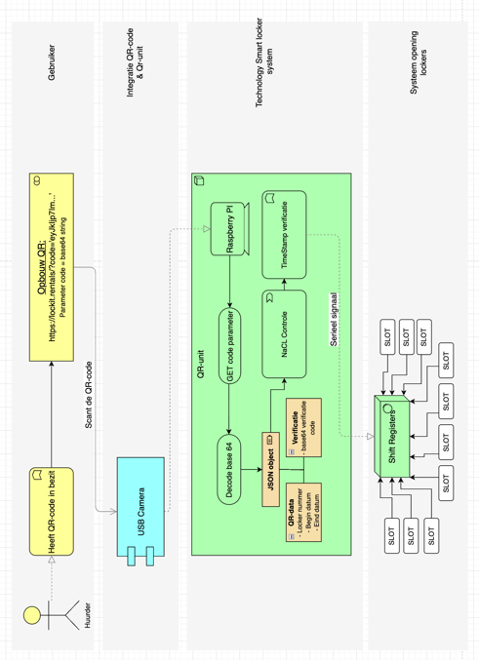
\includegraphics{F16_schemaWerking.png}
    \captionsetup{justification=ce/brntering, singlelinecheck=false}    
    \caption{Een schematische voorstelling  hoe een QR-unit operationeel te werk gaat.}
    \label{fig:schemaWerkingUnit}
\end{figure}

\subsubsection{Stap 1: QR-code in bezit}

De huurder heeft zich succesvol geregistreerd en een toegangscode verkregen. 

\subsubsection{Stap 2: QR-code scannen}

De QR-code die alvorens is aangemaakt wordt uitgelezen met een USB camera. De software van de camera draait rechtstreeks op de Rasberry PI. 
 \begin{lstlisting}[language=Python, caption={Het uitvoerbare script van de QR-unit, die de toegangscode zal uitlezen.}, label={lst:pythonPrimary1}, numbers=left]
    from datetime import datetime, timedelta
    import time
    import cv2
    
    camera = cv2.VideoCapture(0)
    
    try:
        global data
        data = ""
        global stamp
        stamp = datetime.now()
        print('reading camera...', end='\r')
        frame_rate = 3
        prev = 0
        while True:
        # Read current frame
        if camera.isOpened():
            time_elapsed = time.time() - prev
            ret, frame = camera.read()
            if time_elapsed > 1./frame_rate:
            prev = time.time()
            im=decodeCam(frame)
    except KeyboardInterrupt:
    print('interrupted!')
\end{lstlisting}
Lijn 5 \ref{lst:pythonPrimary1}: Het definiëren van de camera zodat hij kan gebruikt worden om de QR-code waar te nemen. \\    
Lijn 7 – 22 \ref{lst:pythonPrimary1}: Een oneindige lus waarin de camera constant probeert om QR-codes te scannen. Als hij een QR-code opmerkt, zal hij deze vertalen en zal de methode ‘decodeCam’ opgeroepen worden. De gescande afbeelding die voorgesteld wordt als QR-code zal hierin meegegeven worden.\\

\subsubsection{Stap 3: Raspberry PI leest QR-code}
Een Raspberry PI is een kleine maar krachtige mini computer die allerlei berekeningen kan uitvoeren \autocite{Richardson2013}. Deze bevat alle logica die uitgevoerd wordt na het scannen van de QR-code.  De aangesloten USB camera zal de afbeeldingen proberen te verwerken zodat de gekoppelde locker geopend wordt. Niet alleen het uitvoerbaar script draait op de Raspberry PI ook een server die alle verzoeken afhandelt. Indien er een QR-code goed wordt uitgelezen, stuurt het proces een verzoek naar de node.js server, die op zijn beurt de controle overneemt.

   \begin{lstlisting}[language=Python, caption={Het primaire uitvoerbare script van de QR-unit.}, label={lst:pythonPrimary2}, numbers=left]
    import cv2
    import pyzbar.pyzbar as pyzbar
    from datetime import datetime, timedelta
    import requests
        
    def decodeCam(image):
        try:
            gray = cv2.cvtColor(image, cv2.COLOR_BGR2GRAY)
            barcodes = pyzbar.decode(gray, symbols=[pyzbar.ZBarSymbol.QRCODE])
            global data
            global stamp
            for barcode in barcodes:
                barcodeData = barcode.data.decode()
                barcodeType = barcode.type
                if barcodeData != data or stamp + timedelta(days=0, seconds=5) < datetime.now():
                    print("["+str(datetime.now())+"] Type:{} | Data: {}".format(barcodeType, barcodeData))
                    res = requests.post('http://localhost:5000/qr-code', json = {'tag': barcodeData })
                    print(res)
                    data = barcodeData
                    stamp = datetime.now()
                    return image
        except Exception as e:
        print(e)
    
\end{lstlisting}

Lijn 8 \ref{lst:pythonPrimary2}: Cv2 is een software pakket dat visuele afbeeldingen kan laden en verwerking in de taal Python. Het pakket verwijdert de resulterende grijsvariabelen die in de invoerafbeelding zitten. Dit betekent dat als de huurder een afbeelding scant hij enkel specifieke kleuren zal overhouden. Hierdoor kan het primaire Python script verder werken met één informatiekanaal, in plaats van meerdere in geval van een kleurenafbeelding \autocite{developmentteam}.\\
Lijn 9 \ref{lst:pythonPrimary2}: PyZbar is een andere bibliotheek die instaat om de QR-codes te gaan detecteren van de grijswaardenafbeelding die zonet met Cv2 bekend zijn gemaakt \autocite{Huang2022}\\
Lijn 17 \ref{lst:pythonPrimary2}: De Rasberry PI zal een request sturen naar de Node.js server die rechtstreeks draait op de PI. Deze server ontvangt een parameter waarin de QR-code data zit.\\


\subsubsection{Stap 4: Parameter code}

Bij het doorsturen van de verkregen URL via de node.js server heeft de applicatie enkel nood aan de parameter 'Code'\autocite{Weir2012}.  Die base64 string wordt uit de link gefilterd door de URL op te splitsen. 

\begin{lstlisting}[language=Python, caption={Python script om parameter code uit de link te halen.}, label={lst:pythonLinkSplitting}, numbers=left]
    router.post('/qr-code', (request, response) => {
        try {
            const decryptedData = decryptor.decrypt(request.body.tag);
            console.log(decryptedData);
            
     ...
    
    decrypt: function(url) {
        if (!url) {
            return new Error();
        }
        const data = url.split("code=")[1]
\end{lstlisting}

\subsubsection{Stap 5: Parameter decoderen aan de hand van functie 'Base64'}
Eenmaal dat de base64 string gevonden is, zal dit terug geconverteerd worden naar een \ac{JSON} object. Dit bevat twee objecten. Enerzijds QR-data, waarin drie elementen uitgehaald worden: het lockernummer alsook de begin- en einddatum tot wanneer de QR-code geldig is. Deze tijdstippen worden beide voorgesteld als type Unix. Deze zorgen voor een makkelijke conversie tussen verschillende tijdzones en formaten \autocite{Ritchie1978}. Anderzijds omvat het \ac{JSON} object ook de verificatie code van het encryptie proces dat eerder is uitgewerkt in het code voorbeeld \ref{lst:createCode}. 

\begin{lstlisting}[language=Python, caption={Python code om parameter code te decoderen en informatie op te halen uit het object.}, label={lst:pythonLinkSplitting}, numbers=left]
    const obj = JSON.parse(Buffer.from(data, 'base64').toString('utf8')); 
\end{lstlisting}

\subsubsection{Stap 6: QR-code verifiëren aan de hand van TweetNaCL}

Om de echtheid en correctheid van de QR-code te garanderen moet de ingelezen QR-code gevalideerd worden. De ingelezen QR-code wordt verwerkt en ontcijferd met een zelf gemaakte functie genaamd 'decrypt'. Deze functie zorgt ervoor dat de QR-code omgezet wordt naar een handelbaar formaat. Nadien kunnen we de QR-code gaan valideren met behulp van het extern software pakket TweetNaCL. Voor verdere informatie verwijs ik naar het hoofdstuk \ref{sec:encryptQR-code} met een uitgewerkt voorbeeld in sectie \ref{sec:controleaangemaakteQRcode}. Als de functie geen foutboodschap teruggeeft, kunnen we ervanuit gaan dat deze code zich in een veilige staat bezit.

\begin{lstlisting}[language=Python, caption={Python code om QR-code te verifieren op geldige digitale handtekening.}, label={lst:pythonVerifySigning}, numbers=left]
    router.post('/qr-code', (request, response) => {
        try {
            const decryptedData = decryptor.decrypt(request.body.tag);
            console.log(decryptedData);
            
            const hasErrors = validator.validate(decryptedData, Number(config.unit));
            if (hasErrors) {
                displayError(hasErrors.errorMessage);
                return;
            }
            
            ...
            
            decrypt: function(url) {
                const obj = JSON.parse(Buffer.from(data, 'base64').toString('utf8'));
                
                // Check if the object validates
                if (!nacl.sign.detached.verify(decodeUTF8(JSON.stringify(obj.d)), decodeBase64(obj.v), decodeBase64(publicKey))) {
                    return new Error();
                }
\end{lstlisting}

\subsubsection{Stap 7: Validatie van QR-code op tijd en bijpassende QR-unit}           
        
De validatie functie is gebaseerd op de twee tijdspanne die aanwezig zijn in het aangemaakt \ac{JSON} object. Met deze techniek kan bekeken worden of de gescande QR-code binnen een correcte tijdspanne ligt. Niet enkel controleert hij op correcte geldigheid, ook voert de code hieronder \ref{lst:data-validator} een controle uit of de QR-code wel bij de bijpassende QR-unit hoort.

\begin{lstlisting}[language=Python, caption={Validatie van QR-code op tijd en bijpassende QR-unit.}, label=lst:data-validator, numbers=left]
    const moment = require('moment');
    
    module.exports = {
        validate: function(data, unit) {
            const now = moment(); // create a moment with the current time
            const then = moment.unix(data.t); // create a moment with the other time timestamp in seconds
            const delta = now.diff(then, 'milliseconds'); // get the millisecond difference
            console.log("diff to " + delta)
            // Check if number is in range for this unit (number is not mandatory)
            if (data.n && (data.n < getFirstLockerNumber(unit) || data.n > getLastLockerNumber(unit))) {
                return {errorMessage: 'Locker not in this unit'}
            }
            // Check if after start time
            if (moment().isBefore(moment.unix(data.f))) {
                return {errorMessage: "This code is not yet valid"}
            }
            
            // Check if before end time
            if (moment().isAfter(moment.unix(data.t))) {
                return {errorMessage: "This code is expired"}
            }
            return false;
        }
    }
    
    
    function getFirstLockerNumber(unit) {
        return ((unit - 1) * 128) + 1;
    }
    
    function getLastLockerNumber(unit) {
        return ((unit - 1) * 128) + 128;
    }
    
\end{lstlisting}
\newpage
\subsubsection{Stap 8: Openen van juiste locker door het sturen van serieel signaal} 

Op basis van de correcte originele ontcijferde data kan de server de juiste sloten aansturen. De Raspberry Pi stuurt een serieel signaal naar de verschillende shift registers, die elk op zich verantwoordelijk zijn om een aantal verschillende sloten te besturen.

\begin{lstlisting}[language=Python, caption={Openen van juiste locker of foutboodschap.}, label=lst:pythonPinController, numbers=left]
    if (decryptedData.n) {
        pinController.openLock(calculateExactLock(Number(decryptedData.n), Number(config.unit)));
    } else if(decryptedData.r) {
        pinController.openRange(decryptedData.r.map(l => calculateExactLock(Number(l), Number(config.unit))))
    } else if(decryptedData.u) {
        //universal key scanned
        pinController.openRange(Array.from({length: 128}, (_, i) => i + 1))
    } else if(decryptedData.fu) {
        //force update key scanned
        pinController.update();
        var yourscript = exec('sh ./updater.sh',
        (error, stdout, stderr) => {
            console.log(stdout);
            console.log(stderr);
            if (error !== null) {
                console.log(`exec error: ${error}`);
            }
            if(error || stderr || stdout.toLowerCase().indexOf('offline') > -1) {
                displayError('unit offline');
            }
        });
    }
    
    } catch (e) {
    console.log('foutje: ' + e, e)
    displayError('Not a valid QR code');
    } finally {
    response.send();
    }
\end{lstlisting}

\newpage


\section{Wat is een chatbot}%
\label{sec:chatbot}

De term chatbot is heel snel geëvolueerd doorheen de voorbije jaren. Een chatbot is een "online mens-computer dialoogsysteem met natuurlijke taal" \autocite{Jia2003}. Dit wordt gebruikt om veel systemen te ondersteunen alsook om vragen van klanten automatisch te laten beantwoorden \autocite{Adamopoulou2020}. Ze maken gebruik van artificiële intelligentie die de vraagstelling van klanten analyseren. Op basis van de benodigdheden probeert de chatbot zo goed mogelijk te helpen \autocite{Khanna2015}. Dit concept waarbij de mens de computer om een gunst vraagt, wordt ‘Human-computer interaction’ (HCI) genoemd \autocite{Adamopoulou2020}. De interactie tussen de mens en een gestuurde computer loopt via tekst of stem. De computer probeert één of meerdere talen te begrijpen aan de hand van ‘Natural Language Understanding’ (NLP) \autocite{Khanna2015a}. Deze techniek is ontworpen voor het begrijpen van menselijke noden. Het uiteindelijk doel van de eindgebruiker zal hieruit geëxtraheerd worden.  Chatbots zijn niet enkel gebouwd om conversaties op te vangen of om mensen te entertainen. Deze zijn ook ontworpen voor leer-, informatie- en bedrijfsdoeleinden \autocite{Shawar2007}. 

\subsection{Historie van een chatbot}%
\label{sec:chatbotHistorie}

Het idee van een chatbot werd het eerst gepubliceerd in 1950 \autocite{Turing2009}. Echter bestaat de eerste chatbot genaamd Eliza nog maar sinds 1966 \autocite{Weizenbaum1966}. Deze is ontworpen aan de hand van een simpel patronen overeenkomst en een vooraf aangemaakt antwoorden patroon.  Vanaf dit moment in de geschiedenis begon de functionaliteit en de ontwikkeling van chatbot alsmaar groter te worden \autocite{Brandtzaeg2017}. Zoals getoond in de figuur \ref{fig:graphDocusChatbotAYear} volgens Scopus \autocite{Elsevier2004}, was er grote en snelle groei van interesse in chatbots, zeker na het jaar 2016 \autocite{Adamopoulou2020}.

\begin{figure}[h]
    \centering
    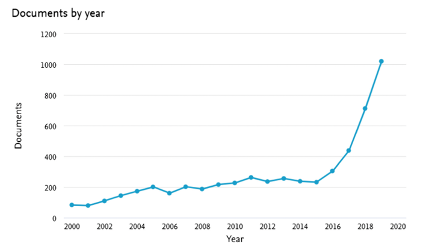
\includegraphics{F17_grafiekChatbotSearches.png}
    \captionsetup{justification=ce/brntering, singlelinecheck=false}    
    \caption{Zoek resultaten in scopus voor de termen ‘chatbot’ of ‘conversation agent’ of ‘conversational interface’ vanaf 2000 tot 2019.}
    \label{fig:graphDocusChatbotAYear}
\end{figure}


\subsection{Architectuur  van een chatbot}%
\label{sec:chatbotArchitectuur}

De start van de menselijke vraag tot een gegenereerde chatbot antwoord wordt voorgesteld als de architectuur van een chatbot. Als illustrerend voorbeeld vragen we als chatbot zijn/haar verloren QR-code op. De huurder heeft een specifieke vraag die de chatbot kan verwerken. Na het krijgen van de huurder zijn bericht zal de ‘Natural Language Understanding’ (NLUs) \autocite{Khanna2015} component de vraag analyseren en classificeren wat de gebruiker zijn intenties zijn \autocite{Tamrakar2021}. Wanneer er een duidelijk geformuleerde vraag gesteld is, kan de chatbot acties ondernemen. In het geval met de verloren QR-code zal hij een API oproep aanspreken om externe informatie op te vragen. Nadien kan de data worden vrijgegeven aan de gebruiker indien de huurder zich juist kan identificeren als het gaat om gevoelige informatie \autocite{Adamopoulou2020}. De architectuur kan voorgesteld worden op figuur \ref{fig:chatbotArchitectuur}.

\begin{figure}[h]
    \centering
    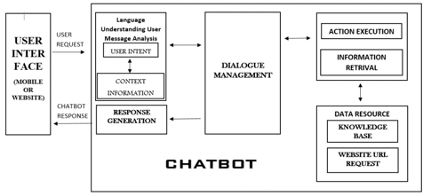
\includegraphics{F18_chatbotArchitectuur.png}
    \captionsetup{justification=ce/brntering, singlelinecheck=false}    
    \caption{Standaard architectuur van een chatbot.}
    \label{fig:chatbotArchitectuur}
\end{figure}

\subsection{Classificatie chatbots}%
\label{sec:chatbotTypes}

Chatbots kunnen geclassificeerd worden door middel van een aantal eigenschappen \ref{fig:chatbotTypes} zoals het interactie level en op welke manier de antwoorden gegenereerd worden \autocite{Nimavat2017}.
Een schematische voorstelling van de classificatie tussen soorten chatbots wordt weergegeven in figuur \ref{fig:chatbotTypes} \autocite{Tamrakar2021}.


\begin{figure}[h]
    \centering
    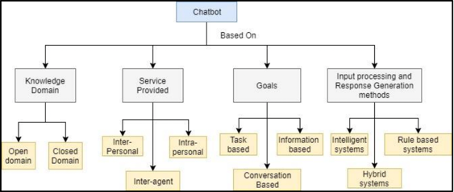
\includegraphics{F19_chatbotClassificatie.png}
    \captionsetup{justification=ce/brntering, singlelinecheck=false}    
    \caption{Classificaties en soorten van een chatbot.}
    \label{fig:chatbotTypes}
\end{figure}

Chatbots worden onderverdeeld in categorieën door gebruik te maken van enkele parameters. Voorbeelden van parameters zijn het kennisdomein, dienstverlening, de methode voor het verwerken van de input en het genereren van een antwoord en menselijke hulp en bouwmethode \autocite{Adamopoulou2020}. 

Twee grote categorieën waarin de soort chatbot verschillen zijn open domeinen en gesloten domeinen. Open domein chatbots vertellen ons meer over algemene onderwerpen die een zo goed mogelijk antwoord geven op de vraag van de gebruiker. Gesloten domein chatbots werken aan de hand van algemene domein kennis van de chatbot \autocite{Adamopoulou2020}. Nadelig hieraan is dat niet alle vragen even goed kunnen beantwoord worden \autocite{Kucherbaev2018}.

Een verdere onderscheid van chatbots zijn de soorten aangeboden diensten: ‘Interpersonal, ‘Intrapersonal en ‘Inter-agent’. Met een ‘Intrapersonal’ service communiceert hij de gekende informatie zoals openingsuren van een winkel, of trein boekingen met de eindgebruiker \autocite{Adamopoulou2020}. ‘Intrapersonal’ bots proberen de gebruiker te verstaan en te helpen zoals een echte mens. Deze gaan opzoek naar persoonlijke domein data van de gebruiker. Als laatste onderverdeling van dienstverlening bestaat de ‘Inter-agent’ chatbot. Deze bots communiceren met andere bots om hun informatie te delen. Op deze manier kunnen ze het best passende antwoorden schenken \autocite{Nimavat2017}.

De bots hebben altijd een specifiek doel. Daarvoor wordt er gekeken naar wat de chatbot wil bereiken. Wil de chatbot informatie verschaffen aan de gebruiker aan de hand van vaste middelen dan spreken we over informatieve chatbots. Bij het geval van ‘Task based’ zal de chatbot effectief een taak uitvoeren aan de hand van specifieke eisen. Als meest gebruikte vorm van chatbot is er de chat gebaseerde of conversatie chatbot. Deze is puur gericht om het juiste antwoord te verschaffen op de gestelde vraag (\autocite{Nimavat2017} \autocite{Adamopoulou2020}. 

De drie modellen die geklasseerd onder ‘respons en generation method’ stellen methodes voor die de vraagstelling in acht neemt en genereert een gepast antwoord. Als eerste bestaat er de ‘Rule based’ model. Deze bots worden zo getraind en geprogrammeerd om op specifieke zoektermen de juiste vooraf gedefinieerde antwoorden te verschaffen. De toepassing van \ac{FAQ} bot is hiervan een voorbeeld. Deze bot verschilt maar nauwelijks ten opzichte van een ‘Retrieval based model, wat meer flexibiliteit geeft. Het analyseert verschillende mogelijke bronnen aan de hand van ‘APIs’. Het laatste model is ‘Generative’.  Dit model is gebaseerd om op vorige berichten een antwoord te voorzien. Dit is het meest krachtigste model en het meest complexe om te programmeren en te trainen \autocite{Adamopoulou2020} \autocite{Hien2018}.

Voor het aanmaken van een chatbot die verloren QR-codes zal terugwinnen, kan de chatbot onderverdeeld worden in een juiste classificatie. De technologie die van toepassing is op Lockit Rentals zal gebaseerd zijn op een gesloten domein. Hierdoor zal de chatbot niet op alle vragen een gepast antwoord kunnen geven. De chatbot zal op vooraf geprogrammeerde vragen de juiste informatie geven. Het dialoog systeem zal de antwoorden verschaffen aan de hand van een ‘intrapersonal service’. Hij verzamelt correct gefilterde informatie uit de databank en verschaft deze aan de eindgebruiker. De chatbot voert een specifieke opdracht uit waardoor de klant weer toegang krijgt tot zijn eigen persoonlijke locker. De laatste classificatie maakt gebruik van rule based methodes om de chatbot zo goed mogelijk te ontwikkelen. Deze regels zijn vooraf gedefinieerd en begeleiden de klant in de juiste richting waardoor het terugkrijgen van een verloren QR-code een vereenvoudigd proces wordt.
\subsection{Platformen om chatbots te bouwen}%
\label{sec:chatbotBouwen}

De manieren om een chatbot te ontwikkelen hangt af van enkele factoren. Het keuze ontwerp wordt beïnvloed door welk type bot en door welke specifieke verwachtingen van de gebruiker \autocite{Rahman2017}.

Chatbots die niet ontworpen zijn aan de hand van een platvorm behoren tot de categorie ‘No coding chatbot’ \autocite{Tamrakar2021}. Een andere techniek dat gehanteerd wordt om chatbots te ontwikkelen zijn platvormen die vooraf geprogrammeerde algoritmes en modules bevatten. Het gebruik van deze platvormen zijn eenvoudig omdat er geen kennis van programmeervaardigheden vereist zijn. Deze platvormen worden gebruikt voor het ontwerpen van kleine en versimpelde chatbots  \autocite{Rahman2017}. Enkele voorbeelden van veelgebruikte ‘no coding chatbot’ platvormen zijn Chatfuel, manychat and Mothian.ai, botpress, etc.  \autocite{Rahman2017}. 
Chatbots worden ook ontwikkeld door platvormen van technologiegiganten zoals Google, Amazon, Microsoft, etc. \autocite{Gkikas2021}. Deze platvormen zijn robuust van aard en worden gebruikt om complexe bots te ontwerpen. De robuuste structuur heeft als gevolg dat er een conversatie stroomdiagram moet worden aangebracht op het platvorm \autocite{Tamrakar2021}. In deze diagrammen worden er verschillende stappen of interacties tussen een gebruiker en chatbot gedefinieerd. Deze vormen paden die de gebruiker kan nemen bij het stellen van vragen. Dit stroomdiagram zorgt ervoor dat de verzoeken van de gebruiker nooit verkeerd of slecht geïnterpreteerd kunnen worden.  De ontwikkelaars van de bot zullen aan de hand van deze diagram de chatconversatie kunnen structureren en nauwkeurig gaan controleren \autocite{CotyM.CollinsColumbus2019}. Voorbeelden van technologiegiganten chatbot platvormen zijn Google DialogFlow, Facebook’s Wit.ai, Miocrosoft’s LUIS, Aamzon’s Lex en IBM’s Watson, etc \autocite{Tamrakar2021}.





